\chapter{通信网中的流量优化}
\section{一般性问题}
\subsection{可行流及其优化问题
}
\subsubsection{可行流}
流量的两个特性
\begin{itemize}
	\item 非负性和有限性
	\item 连续性
\end{itemize}
满足前述限制条件的流称为可行流
\subsubsection{问题}
\begin{itemize}
	\item 最大流问题
	\item 最佳流或最小费用流问题
\end{itemize}
\section{最大流问题}
\textbf{源宿端达到最大流量的充分必要条件},从vs到vt的每一条边上至少有一个饱和的前向边或一个零流的反向边

\subsection{M算法}
采用DFS和BFS均可做。
\begin{figure}[H]
	\centering
	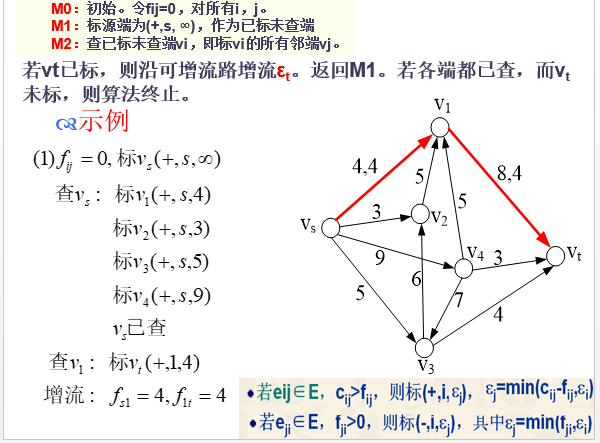
\includegraphics[width=0.7\linewidth]{figures/screenshot083}
	\caption{}
	\label{fig:screenshot083}
\end{figure}
\subsubsection{M算法的几点推广
}
\begin{itemize}
	\item 端容量问题
	\item 多源多宿情况
	\item 求结合度(最小割边集的边数)
\end{itemize}


\subsection{最佳流问题}
如果每条边eij各赋予各自的费用系数aij,那么当总流量Fst相同时,各种可行流的费用可以不同;因此,有时需寻找满足流量要求的最小费用的可行流,例如传送某一信息流时寻找最小费用的路由,以达到最佳的流量分配。\\
\textbf{每条边具有费用系数,当总流量固定时总会有费用最小的路由}

\subsubsection{N算法}
负价环:补图上若存在一个有向环,\textbf{环上各边的费用aij之和是负数},则称此环为负价环。\\
\textbf{如何补图?元祖结构}\\
正向:剩容量,$ a_{ij} $\\
反向:流量,$ -a_{ij} $\\
\vspace{2pt}
步骤:
\begin{enumerate}
	\item 随便找个满足总流量的流量图
	\item 按照补图元祖进行补图
	\item 在补图上寻找负价环,增流值为$ min\{c_{ij}\} $,但是注意增流方向,将这个值增到可行流图上。
	\item 重复前两步,直到找不到负价环
\end{enumerate}
\begin{figure}[H]
	\centering
	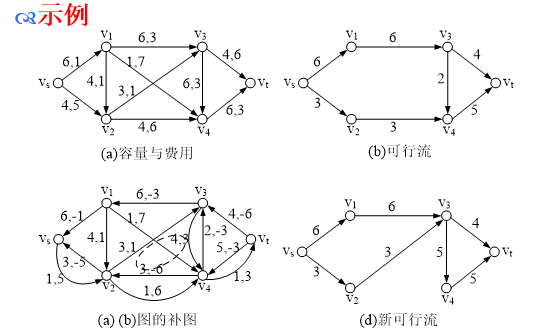
\includegraphics[width=0.7\linewidth]{figures/screenshot084}
	\caption{}
	\label{fig:screenshot084}
\end{figure}
图的容量和费用图是不会发生改变的,改变的是可赠流。

\section{线性规划}
求解线性规划问题就是系统\textbf{地搜索超平面多面体的顶点},以达到f最大。这种方法通常称为\textbf{单纯形法}。
